\section{Results}

Show data from first potentiostat lab (graphs). Explain that we did salenize and platenize. Then talk about how we manufactured wafers and tried to test them. We had trouble getting this to work. Explain why. 

For potentiostat, we used a resistor to test its functionality (gui of graphs). 


\begin{figure}[h]
\begin{center}
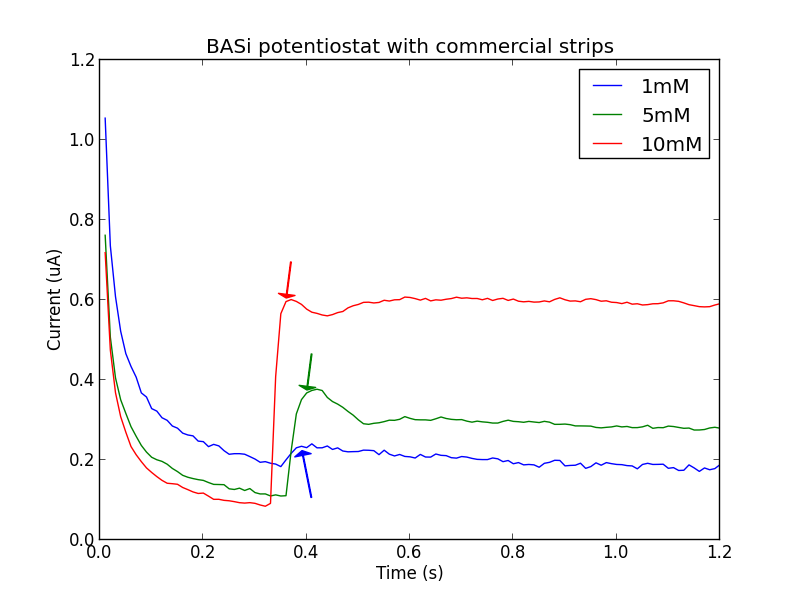
\includegraphics[width=3.5in]{../figures/basi.png}
\end{center}
\caption{Current vs. time plot for three different concentrations of glucose. These tests were done using a BASi potentiostat and commercial electrode strips. The arrow indicate responses to glucose being added to the solution.}
\end{figure}

\begin{figure}[h]
\begin{center}
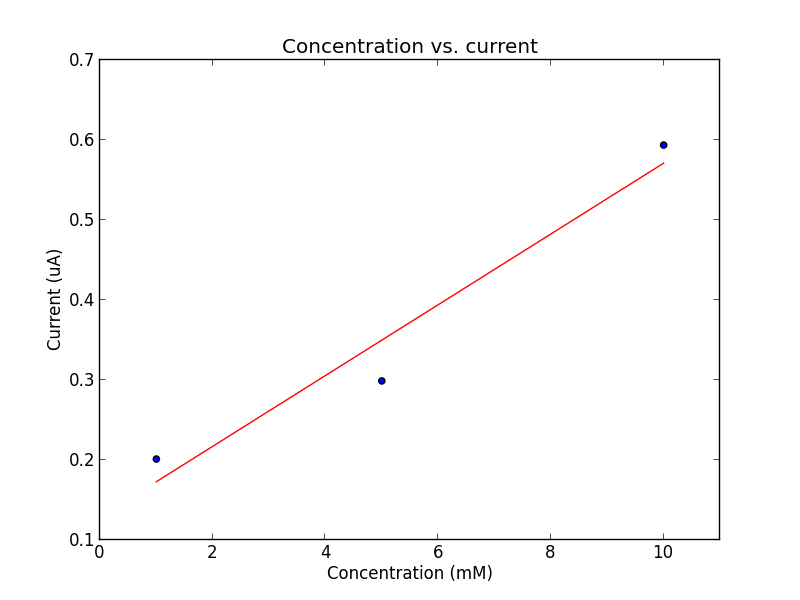
\includegraphics[width=3.5in]{../figures/CI.png}
\end{center}
\caption{Glucose concentration vs. current plot for three different concentrations of glucose. These tests were done using a BASi potentiostat and commercial electrode strips. Each data point is an average of currents after glucose was introduced.}
\end{figure}

\begin{figure}[h]
\begin{center}
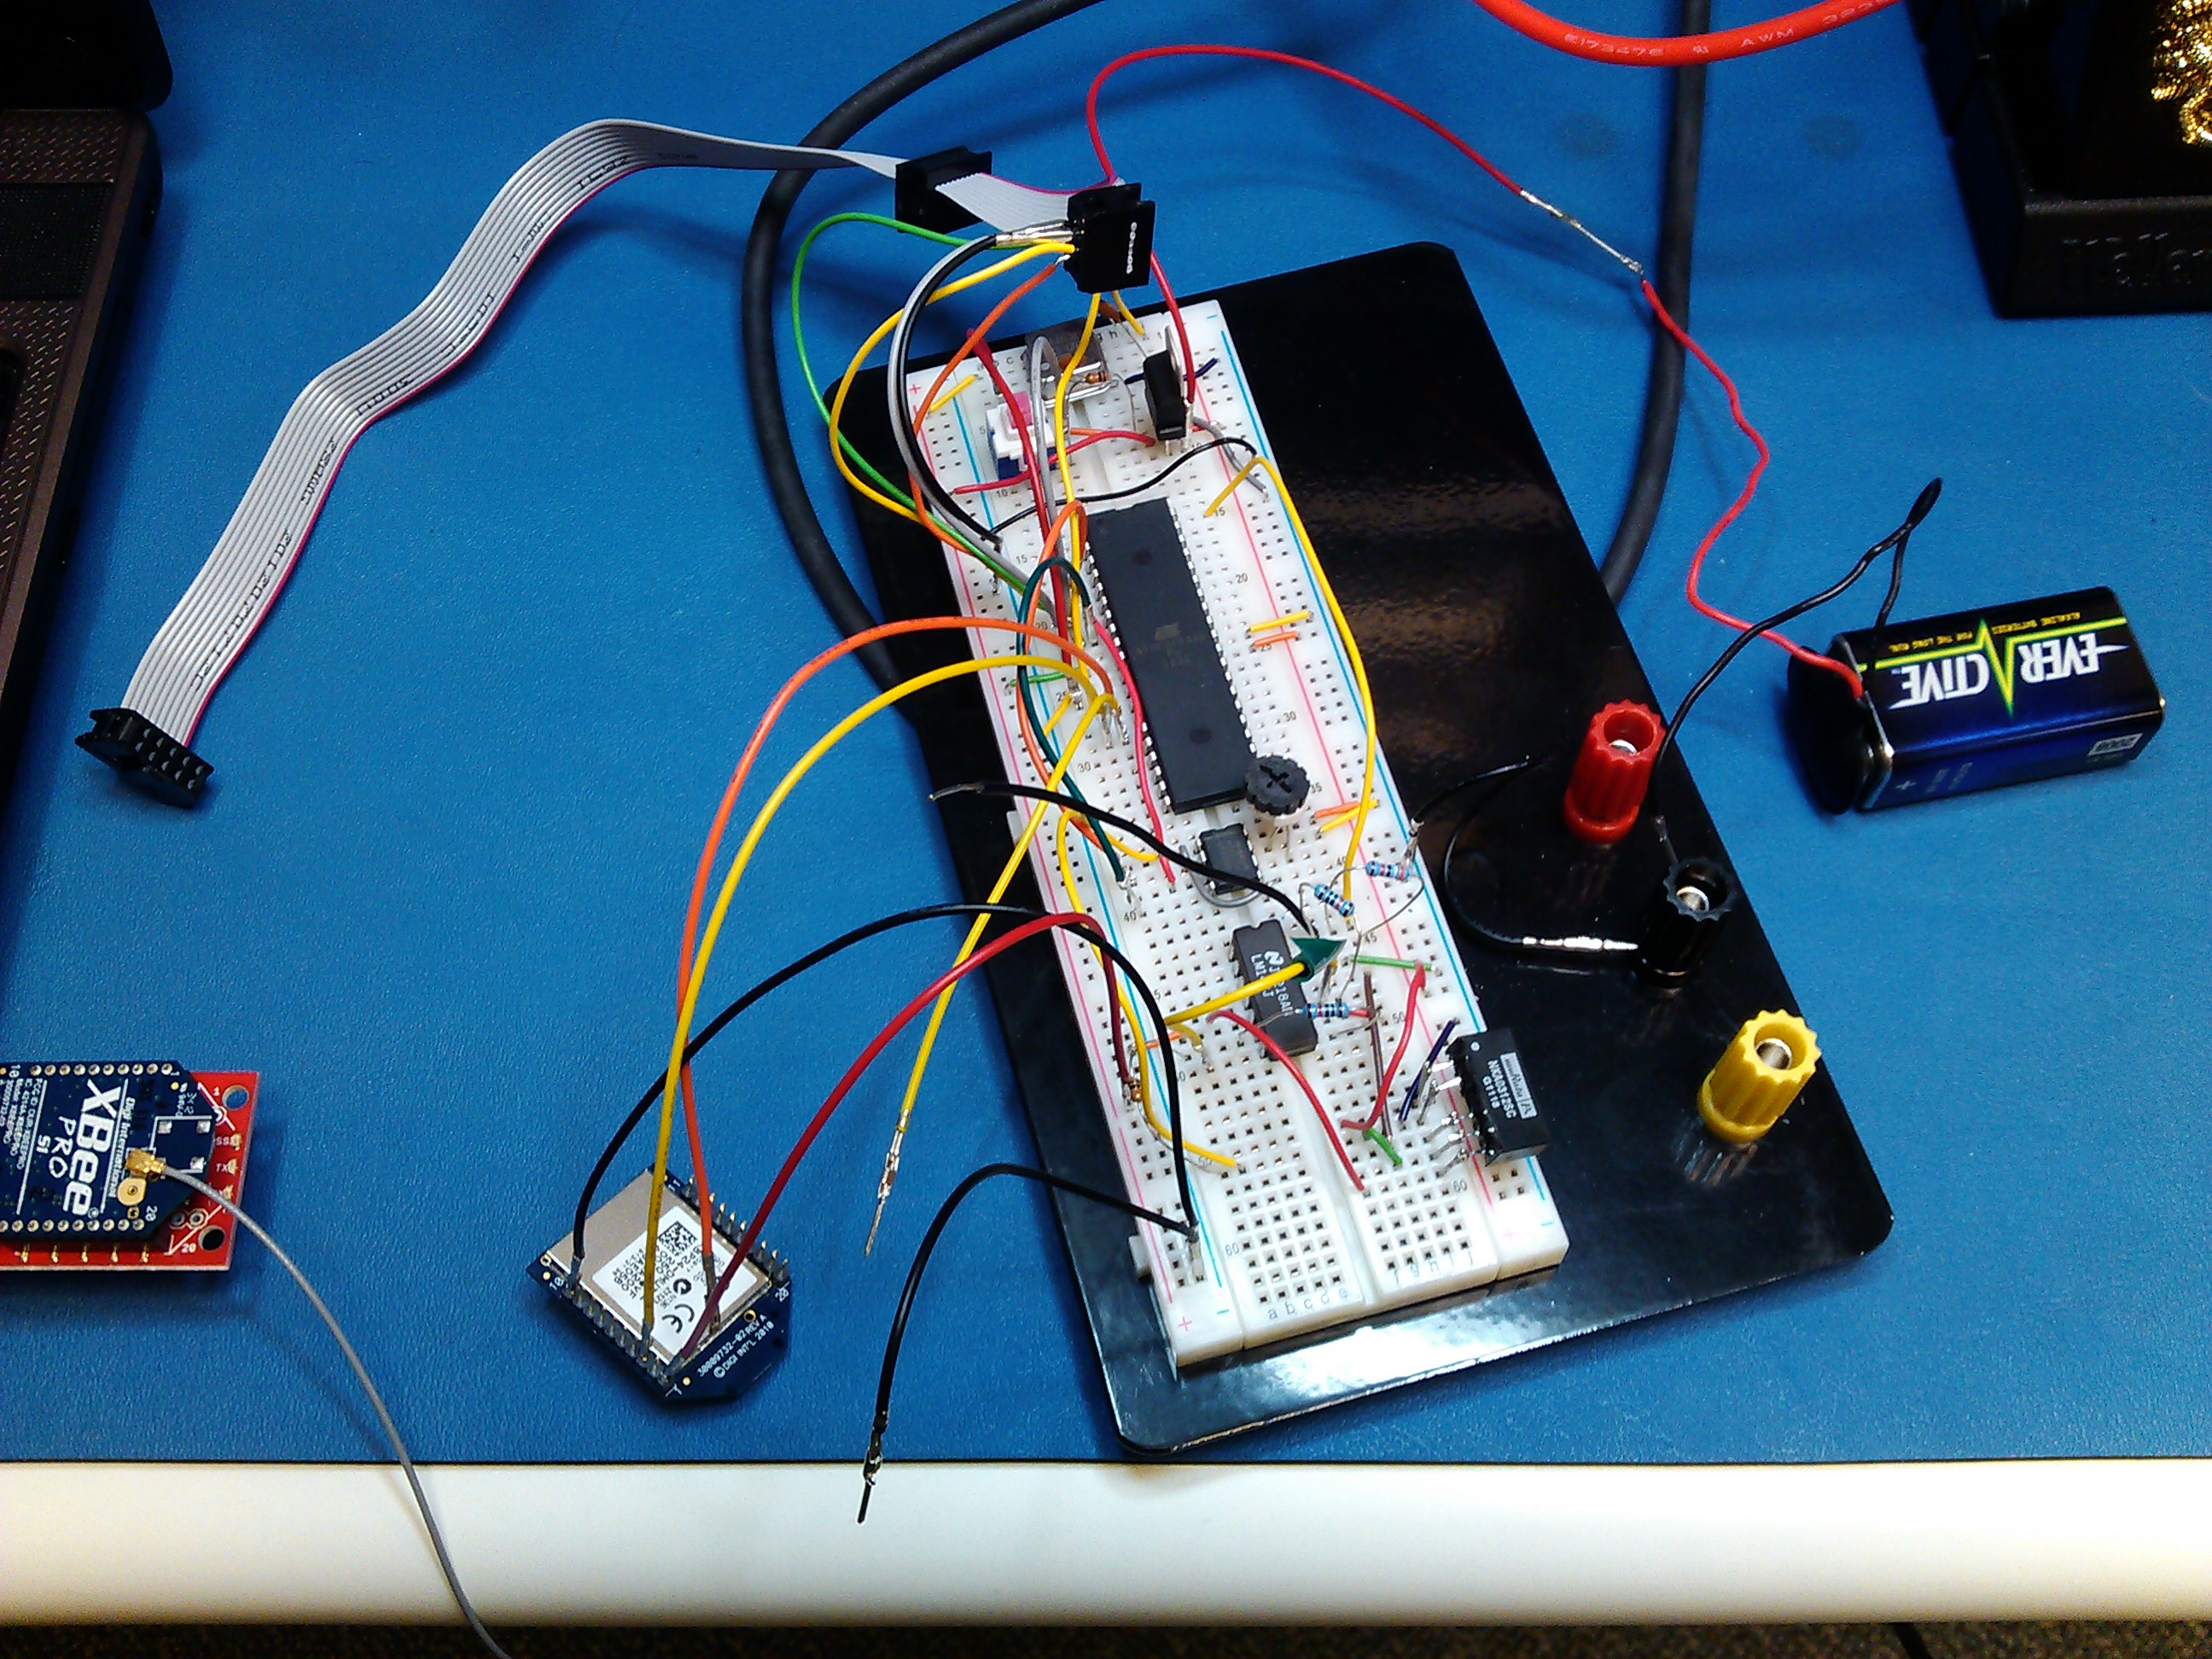
\includegraphics[width=3.5in]{../figures/board.jpg}
\end{center}
\caption{Picture of our system on a breadboard. The system can run off a 9V battery and communicates with a PC via XBee radio.}
\end{figure}
 
\begin{figure}[h]
\begin{center}
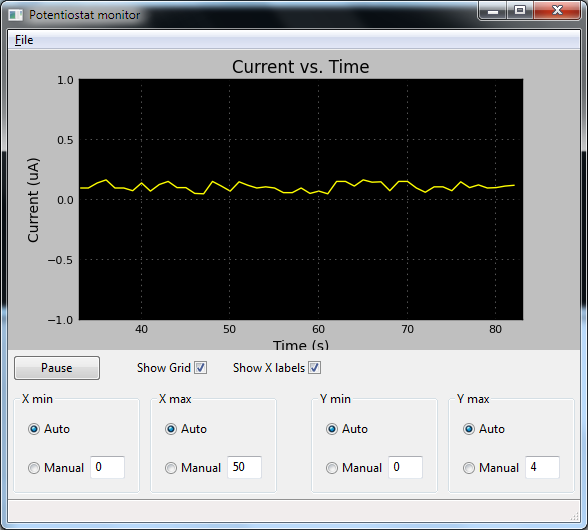
\includegraphics[width=3.5in]{../figures/1Mohm_0,1uA_6,8Mohm.png}
\end{center}
\caption{Low range}
\end{figure}

\begin{figure}[h]
\begin{center}
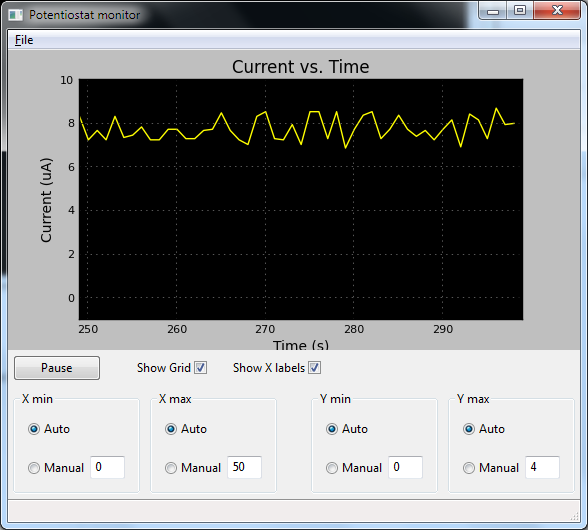
\includegraphics[width=3.5in]{../figures/1Mohm_8uA_680KOhm.png}
\end{center}
\caption{Mid range}
\end{figure}

\begin{figure}[h]
\begin{center}
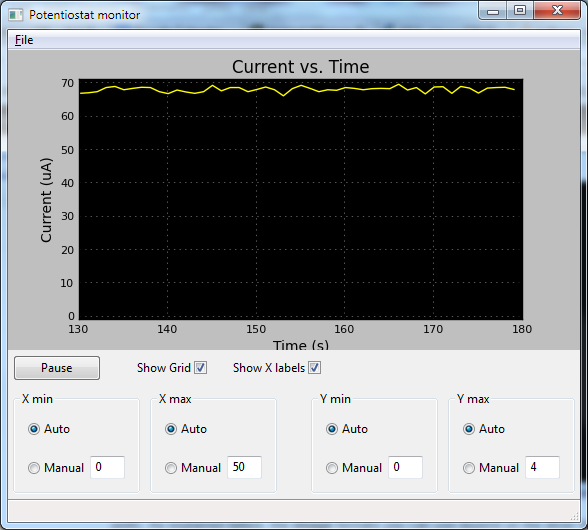
\includegraphics[width=3.5in]{../figures/10KOhm_70uA_39KOhm.png}
\end{center}
\caption{Upper range}
\end{figure}
